\documentclass{article}

\usepackage{graphicx}
\usepackage{tikz}
\usepackage{tikzsymbols}
\usetikzlibrary{calc,patterns,shapes.geometric}
\pagestyle{empty}
\usepackage[margin=0pt]{geometry}
\geometry{papersize={14in,12in}}

\def\centerarc[#1](#2)(#3:#4:#5){\draw[#1] ($(#2)+({#5*cos(#3)},{#5*sin(#3)})$) arc (#3:#4:#5);}

\begin{document}
	\begin{figure}
		\centering
		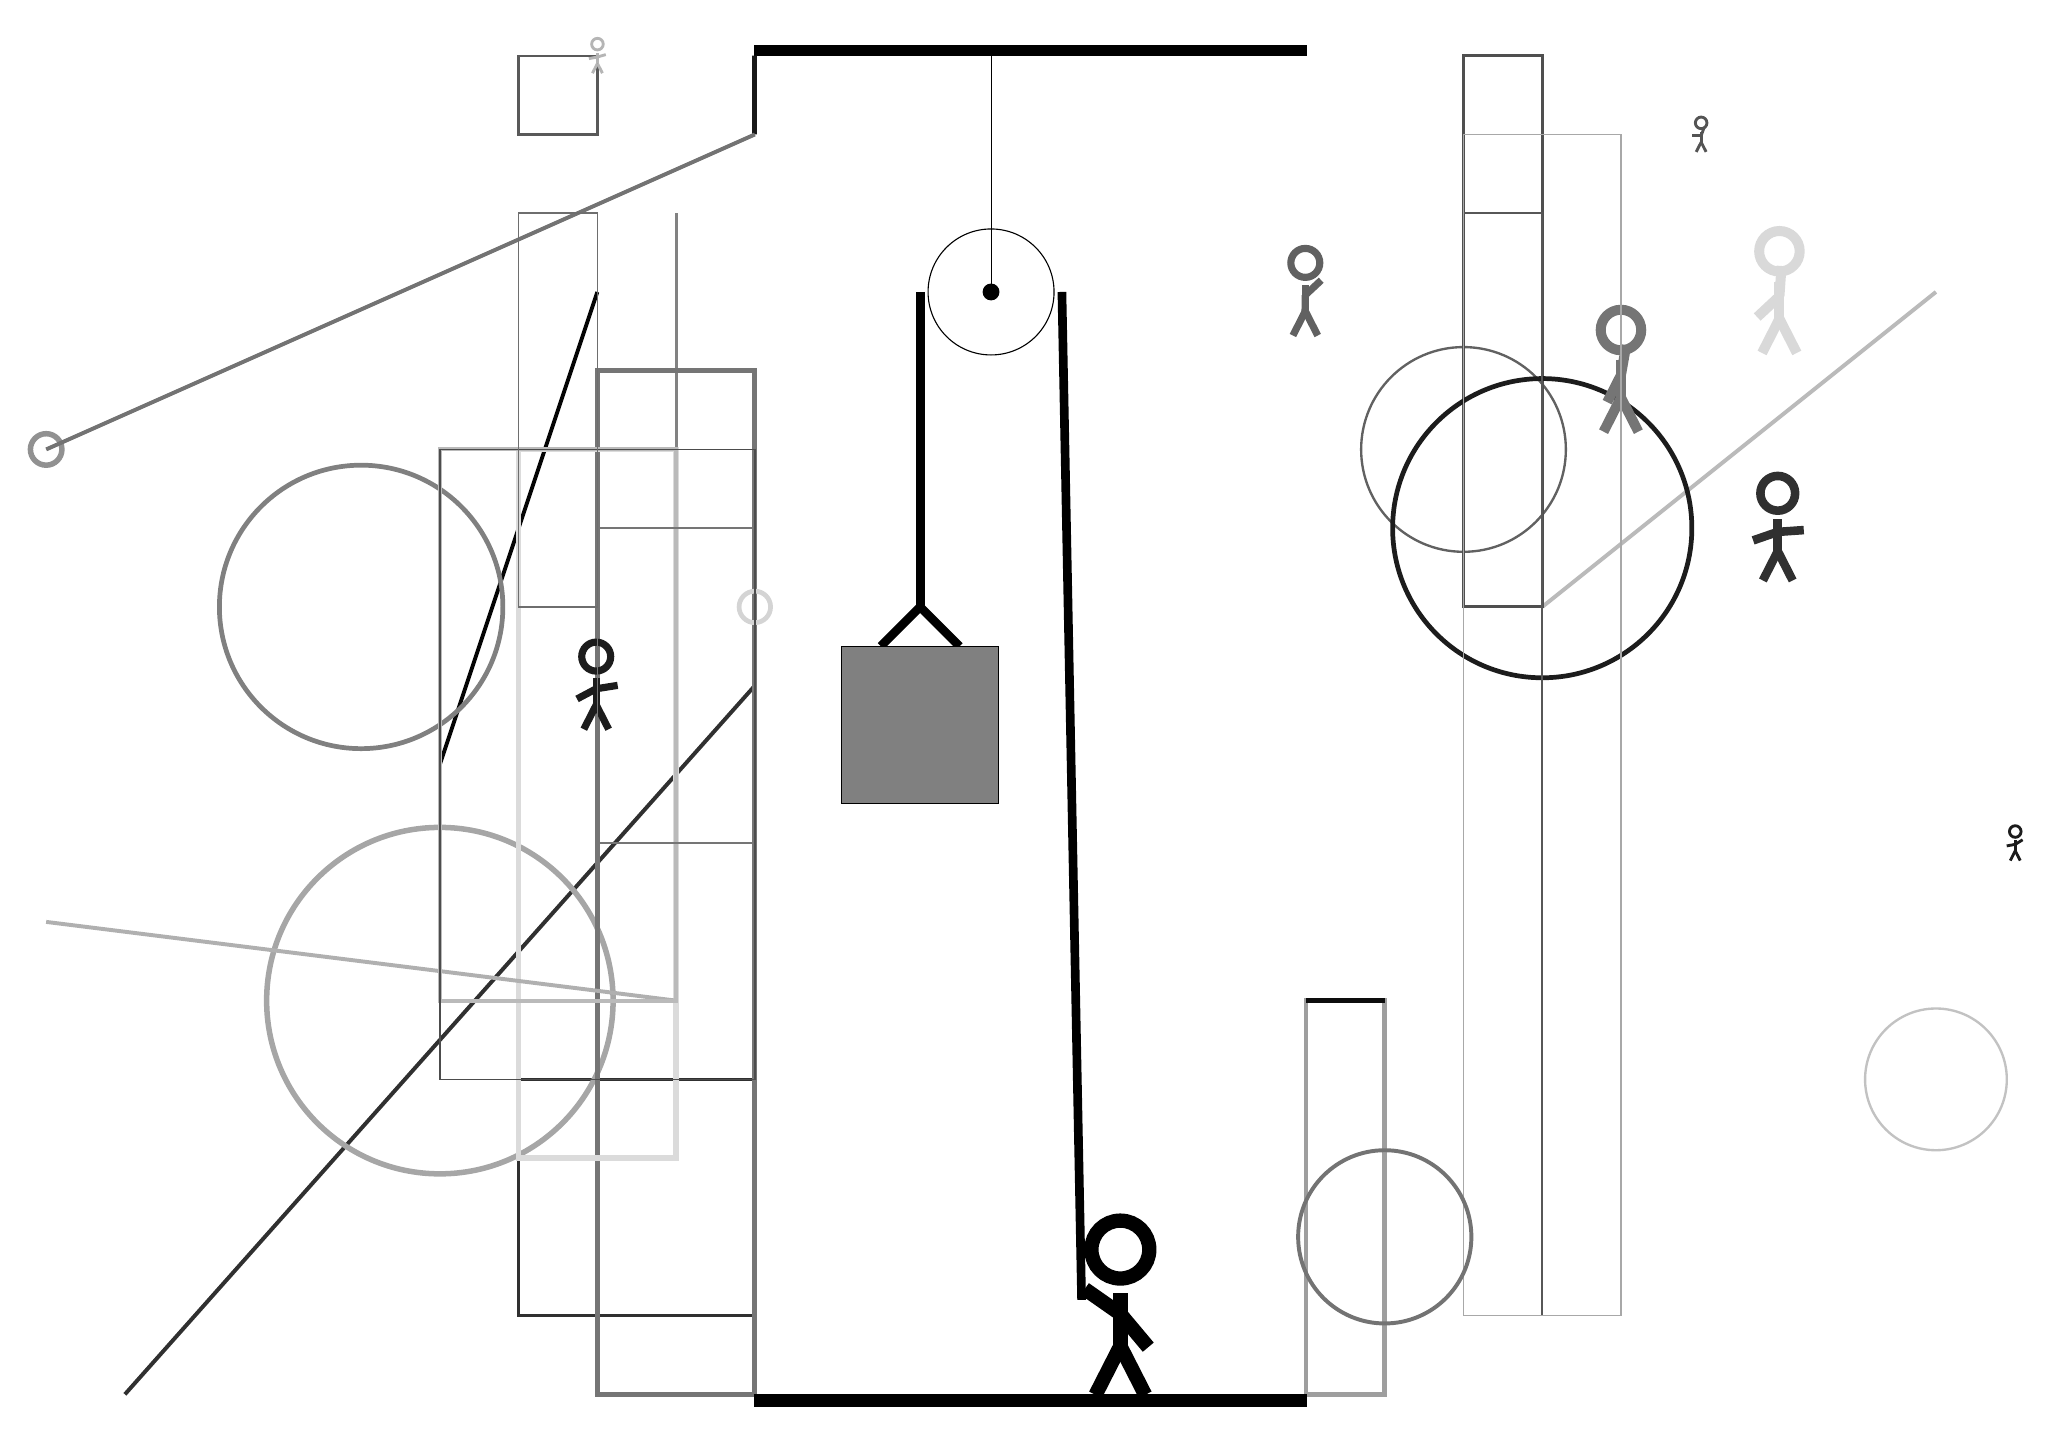
\begin{tikzpicture}
			%%%%% START %%%%%
			
			\draw[fill=black] (-2, 14) rectangle (5, 14.125);
			
			\draw (1, 11) circle (0.8);
			\draw[fill=black] (1, 11) circle (0.1);
			\draw (1, 14) -- (1, 11);
			
			\draw[line width=1.1mm] (-0.4, 6.5) -- (0.1, 7.0) -- (0.6, 6.5);
			\draw[fill=black!50] (-0.9, 6.5) rectangle (1.1, 4.5);
			
			\draw [line width=0.3mm, color=black!62](7, 9) circle (1.3);
			
			\draw[line width=0.5mm, color=black!27](8, 7) -- (13, 11);
			\draw [line width=0.7mm, color=black!43](-11, 9) circle (0.2);
			\draw[line width=0.5mm, color=black!98](-6, 5) -- (-4, 11);
			
			\draw[line width=0.4mm, color=black!69] (7, 14) rectangle (8, 7);
			
			\draw [line width=0.3mm, color=black!24](13, 1) circle (0.9);
			\draw [line width=0.6mm, color=black!50](-7, 7) circle (1.8);
			
			\node[line width=0.6mm, color=black!67] at (10, 13) {\Strichmaxerl[2][0][70]};
			\draw[line width=0.4mm, color=black!81] (-2, -2) rectangle (-5, 1);
			\draw[line width=0.5mm, color=black!81](-2, 6) -- (-10, -3);
			\draw [line width=0.6mm, color=black!89](8, 8) circle (1.9);
			
			\draw[line width=0.5mm, color=black!58] (-4, 9) rectangle (-5, 2);
			\draw[line width=0.2mm, color=black!66] (7, 12) rectangle (8, -2);
			
			\node[line width=0.5mm, color=black!54] at (9, 10) {\Strichmaxerl[7][63][80]};
			\draw [line width=0.7mm, color=black!35](-6, 2) circle (2.2);
			\draw[line width=0.4mm, color=black!49] (-3, 7) rectangle (-3, 12);
			\draw[line width=0.6mm, color=black!54] (-2, 10) rectangle (-4, -3);
			\node[line width=0.6mm, color=black!89] at (-4, 6) {\Strichmaxerl[5][28][9]};
			\draw[line width=0.7mm, color=black!14] (-3, 0) rectangle (-5, 9);
			\node[line width=0.3mm, color=black!15] at (11, 11) {\Strichmaxerl[7][43][86]};
			\draw[line width=0.6mm, color=black!90] (-2, 14) rectangle (-2, 13);
			\draw[line width=0.3mm, color=black!65] (-4, 14) rectangle (-5, 13);
			\draw[line width=0.6mm, color=black!38] (5, 2) rectangle (6, -3);
			\node[line width=0.5mm, color=black!62] at (5, 11) {\Strichmaxerl[5][89][43]};
			\node[line width=0.5mm, color=black!29] at (-4, 14) {\Strichmaxerl[2][11][16]};
			\draw[line width=0.6mm, color=black!95] (6, 2) rectangle (5, 2);
			
			\draw[line width=0.5mm, color=black!31](-3, 2) -- (-11, 3);
			\draw [line width=0.6mm, color=black!17](-2, 7) circle (0.2);
			\draw[line width=0.5mm, color=black!27] (-3, 2) rectangle (-6, 9);
			\node[line width=0.5mm, color=black!89] at (14, 4) {\Strichmaxerl[2][10][32]};
			\draw[line width=0.2mm, color=black!34] (7, 13) rectangle (9, -2);
			
			\draw [line width=0.5mm, color=black!55](6, -1) circle (1.1);
			\draw[line width=0.2mm, color=black!54] (-2, 4) rectangle (-4, 8);
			\draw[line width=0.2mm, color=black!70] (-2, 9) rectangle (-6, 1);
			\draw[line width=0.5mm, color=black!55](-2, 13) -- (-11, 9);
			\draw[line width=0.2mm, color=black!57] (-4, 7) rectangle (-5, 12);
			
			\node[line width=0.4mm, color=black!81] at (11, 8) {\Strichmaxerl[6][19][4]};
			
			
			\draw[line width=1.1mm] (0.1, 11) -- (0.1, 7.0);
			\centerarc[line width=1.1mm](1, 11)(0:180:0.9);
			\draw[line width=1.1mm](1.9, 11) -- (2.15, -1.8);
			
			\node at (2.6, -1.9) {\Strichmaxerl[10][-35][-50]};
			
			\draw[fill=black] (-2, -3) rectangle (5, -3.15);
			
			%%%%% END %%%%%
		\end{tikzpicture}
	\end{figure}	
\end{document}